% =====================================================================
%  chunks/ch03f.tex —— 原书 p.79–90（PDF 86–97）
%  第 3 章 §6 带结构群的单纯丛与胞腔丛。障碍。万有对象。
%  上同调运算。Steenrod 代数。Adams 谱序列（上）
% =====================================================================
% [原文 p.79]
此外，若 $p>2$，则 $n-r$ 为偶数。对于复形对 $(K,L)$ 范畴中的同调 $n$-圆盘，也有类似的结果。（所谓 $\Z/p$-同调 $n$-球面，是指对所有 $j$ 都满足 $H_j(K;\Z/p)\cong H_j(S^n;\Z/p)$ 的复形 $K$。这个定义也可以用在 $n=-1$ 的情形，此时 $S^n$ 是空集。）

% [Tutor Note: 本块第一句直接以「此外」开头，是因为上一句「……则该作用的不动点集同样是某个维数 $r$ 的 $\Z/p$-同调球面」起始于 p.78 而终于 p.79，按「整句归起始页所在块」的规则已由上一块（ch03e）译完，本块不再重复。]

限于本综述的篇幅，不宜再花更多笔墨讨论有限或紧变换群的纯同调理论以及与之相伴的代数-拓扑技巧，尽管已有若干作者研究过这一课题。下文在讨论「K 理论」、「椭圆算子」与「配边论」时，我们将触及光滑变换的有限群与紧群这一主题。

\section[带结构群的丛与障碍。 万有对象。 上同调运算。 Adams 谱序列]{带结构群的单纯丛与胞腔丛。障碍。万有对象：万有纤维丛与 Eilenberg--MacLane 复形的万有性质。上同调运算。Steenrod 代数。Adams 谱序列}

\takeaway{把「结构群」纳入纤维丛的定义后，延拓问题可由障碍上链及其上同调类刻画；由此得到万有丛的分类定理（定理 6.1）、Eilenberg--MacLane 空间的万有性质（式 (6.6)），以及上同调运算与 Steenrod 代数这一整套代数机器。}

现在我们转而详细阐述一个上面已从同伦观点考察过的概念，即纤维丛。这里的定义将包含一个重要新要素——纤维丛的「结构群」，它自然地作为纤维的自同胚（变换）群的子群出现。设
\[
p:E\longrightarrow B\qquad(\text{纤维为 }F)
\]
是（如第 2 章 §3 所定义的）纤维丛，其中 $E$、$F$、$B$ 都是 CW 复形或单纯复形，投影 $p$ 保持胞腔（单形）。在此背景下，所指定的结构映射假定对底空间 $B$ 的每个胞腔（或单形）$\sigma^n_\alpha$ 的某个开邻域 $U(\sigma^n_\alpha)$ 有定义；于是，在 $p^{-1}(\sigma^n_\alpha)$ 上有
\[
\phi_\alpha:p^{-1}(\sigma^n_\alpha)\longrightarrow\sigma^n_\alpha\times F,
\]
其中到各纤维的限制都是 $F$ 的自同胚。进一步要求：两个胞腔（单形）的公共边界（或面）的某个小开邻域上的衔接函数
\[
\lambda_{\alpha\beta}=\phi_\alpha\circ\phi_\beta^{-1}:U(\sigma^n_\alpha\cap\sigma^m_\beta)\times F\longrightarrow U(\sigma^n_\alpha\cap\sigma^m_\beta)\times F
\]
具有形状
\[
\lambda_{\alpha\beta}(x,y)=(x,\hat\lambda_{\alpha\beta}(x)(y)),
\]
其中 $\hat\lambda_{\alpha\beta}(x)$ 对每个点 $x\in U_{\alpha\beta}=U(\sigma^n_\alpha\cap\sigma^m_\beta)$ 是纤维 $F$ 的一个变换。我们假定所有映射 $\hat\lambda_{\alpha\beta}(x)$ 都属于 $F$ 的一个预先指定的变换群 $G$；群 $G$ 就是纤维丛的结构群
% [Tutor Note: 注意 $\hat\lambda_{\alpha\beta}$ 只定义在底空间的交集 $U_{\alpha\beta}$ 上，而不是在整个 $B$ 上；式中两个上标 $n$、$m$ 允许所交的两个胞腔维数不同，这是本书胞腔丛记号的方便之处。]
% [原文 p.80]
（记该丛为 $(E,B,F,p,G)$）。还要求变换 $\hat\lambda_{\alpha\beta}(x)$、$\hat\lambda_{\beta\gamma}(x)$、$\hat\lambda_{\gamma\alpha}(x)$ 的复合是群 $G$ 的单位元：
\begin{equation}
\hat\lambda_{\alpha\beta}(x)\circ\hat\lambda_{\beta\gamma}(x)\circ\hat\lambda_{\gamma\alpha}(x)\equiv 1, \tag{6.1}
\end{equation}
其中 $x$ 取遍三重交 $U_{\alpha\beta}\cap U_{\beta\gamma}\cap U_{\gamma\alpha}$——即衔接函数 $\hat\lambda_{\alpha\beta}$、$\hat\lambda_{\beta\gamma}$、$\hat\lambda_{\gamma\alpha}$ 的公共定义域——的每一点。于是，纤维丛本质上由映射
\begin{equation}
\hat\lambda_{\alpha\beta}:U_{\alpha\beta}\longrightarrow G \tag{6.2}
\end{equation}
连同条件 (6.1) 所决定。

% [Tutor Note: 条件 (6.1) 与 $\hat\lambda_{\beta\alpha}=\hat\lambda_{\alpha\beta}^{-1}$ 合起来正是 $G$ 值 1-上闭链的通常条件；原书把复合次序写成 $\alpha\beta$、$\beta\gamma$、$\gamma\alpha$，只是为了与三重交 $U_{\alpha\beta}\cap U_{\beta\gamma}\cap U_{\gamma\alpha}$ 的指标顺序一致。]

丛的一个\emph{截面}是指任何满足 $p\circ f=1_B$ 的映射 $f:B\to E$。纤维丛之间的一个\emph{丛映射}（或纤维丛映射，两丛须有相同的纤维 $F$ 与群 $G$）是指
\[
\Phi:(E,B,F,p,G)\longrightarrow(E',B',F,p',G),
\]
它按自然方式由映射 $\Phi:E\to E'$ 与 $\phi:B\to B'$ 给出，并与投影交换，即
\[
\phi\circ p=p'\circ\Phi.
\]
进一步要求 $\Phi$ 保持各纤维，即它在纤维上的限制都是同胚。此外，这些同胚还须在如下确切意义下来自结构群 $G$：底空间 $B$ 的每一点上方，映射
\[
\phi'_{\alpha'}\circ\Phi\circ\phi_\alpha^{-1}:F\longrightarrow F
\]
（其中 $\phi'_{\alpha'}$、$\phi_\alpha$ 分别是丛 $E'$、$E$ 的任意适当结构映射）都应当是来自 $G$ 的同胚。

给定纤维丛 $(E',B',F,p',G)$ 与任意映射 $\phi:B\to B'$，就得到 $B$ 上的一个纤维丛，即\emph{诱导丛} $(E,B,F,p,G)$，以及一个纤维丛映射
\[
\Phi:E\longrightarrow E',\qquad\phi:B\longrightarrow B'.
\]
其构造如下：把 $B$ 上将要定义结构映射 $\phi_\alpha$ 的那些特定开集取作 $B'$ 的特定开集 $U'_\alpha$ 的完全原像 $U_\alpha=\phi^{-1}(U'_\alpha)$（必要时可把它们细化为胞腔的开邻域）。在每个这样的 $U_\alpha$ 上方，令 $p^{-1}(U_\alpha)=U_\alpha\times F$。再用衔接函数 $\lambda_{\alpha\beta}$ 把各乘积空间 $p^{-1}(U_\alpha)$ 粘成 $E$：
\[
\lambda_{\alpha\beta}(x,y)=(x,\hat\lambda_{\alpha\beta}(x)(y)),\qquad x\in U_\alpha\cap U_\beta,\ y\in F,
\]
其中变换 $\hat\lambda_{\alpha\beta}$ 由纤维丛 $(E',B',F,p',G)$ 的变换 $\hat\lambda'_{\alpha\beta}$ 如下定义：
\[
\hat\lambda_{\alpha\beta}(x)=\hat\lambda'_{\alpha\beta}(\phi(x))\in G.
\]

% [原文 p.81]
全空间 $E$ 可以形式地看作 $B\times E'$ 中由满足 $\phi(x)=p'(y)$ 的数对 $(x,y)$ 组成的子集。因此，$B$ 上的诱导丛就是通过 $\phi$ 把 $B'$ 上的纤维丛「拉回」而得到的。

\begin{remark}{}
由条件 (6.1) 容易推知，映射 $\hat\lambda_{\alpha\beta}$ 给出底空间 $B$ 的一个一维上闭链，其系数取值于函数芽层 $\mathcal{F}_G$，该层的函数取值于群 $G$（见 §4）。于是按这种方式，每个纤维丛都对应 $H^1(B;\mathcal{F}_G)$ 中的一个元素，而这一对应给出了以结构群 $G$ 的丛按一维层上同调的分类。然而，这个分类本质上是语言上的或同义反复的，尽管它有时有用，例如当群 $G$ 是 Abel 群时。\hfill$\square$
\end{remark}

如前所述，(6.2) 中映射 $\hat\lambda_{\alpha\beta}$ 的集合唯一决定了丛 $(E,B,F,p,G)$ 的结构。当然，一个给定的拓扑群 $G$ 一般能以许多不同方式实现为某个拓扑空间的自同胚群。底空间同为 $B$、结构群同为 $G$、映射 $\hat\lambda_{\alpha\beta}$ 的集合也相同、但纤维可能不同的纤维丛，称为彼此\emph{相伴}的。显然，一个纤维丛决定了它的全部伴丛的结构。

拓扑群 $G$ 作为某纤维 $F$ 的自同胚群，有一个典范的万有实现：取 $F=G$，让 $G$ 通过（右）平移作用于自身（见图 3.8）：
\begin{equation}
g:G\longrightarrow G,\qquad g(h)=hg,\qquad h,g\in G. \tag{6.3}
\end{equation}
带有这种 $G$-作用的纤维丛 $(E,B,G,G,p)$ 称为\emph{主丛}。这类丛最自然地出现在下述情形：一个拓扑群自由地作用（即 $g(x)=x$ 蕴含 $g=1$）于空间 $E$ 上；此时轨道空间 $E/G$ 扮演底空间 $B$ 的角色，投影就是自然投影 $p:E\to E/G$。事实上不难证明，每个主纤维丛都这样产生：即存在 $G$ 在全空间 $E$ 上的自由作用，使底空间 $B$ 自然地等同于轨道空间 $E/G$，而纤维 $p^{-1}(x)$ 等同于 $G$。

特别重要的是 $G$ 为紧李群、以光滑变换自由作用于光滑流形 $E$、且轨道空间 $B=E/G$ 也是光滑流形的情形。这本质上描述了\emph{光滑纤维丛}的概念，后文将更详细地讨论它。另一个有意义的情形是 $G$ 为离散群；此时主 $G$-丛就是前面考虑过的正则覆叠空间。

\begin{definition*}{6.1}
若纤维丛 $(E,B,F,G,p)$ 的相伴主丛 $(E',B,G,G,p)$ 的全空间 $E'$ 可缩，则称该纤维丛是\emph{万有的}。
\end{definition*}

这个定义的意义将在下面显现。

% [原文 p.82]
\begin{center}
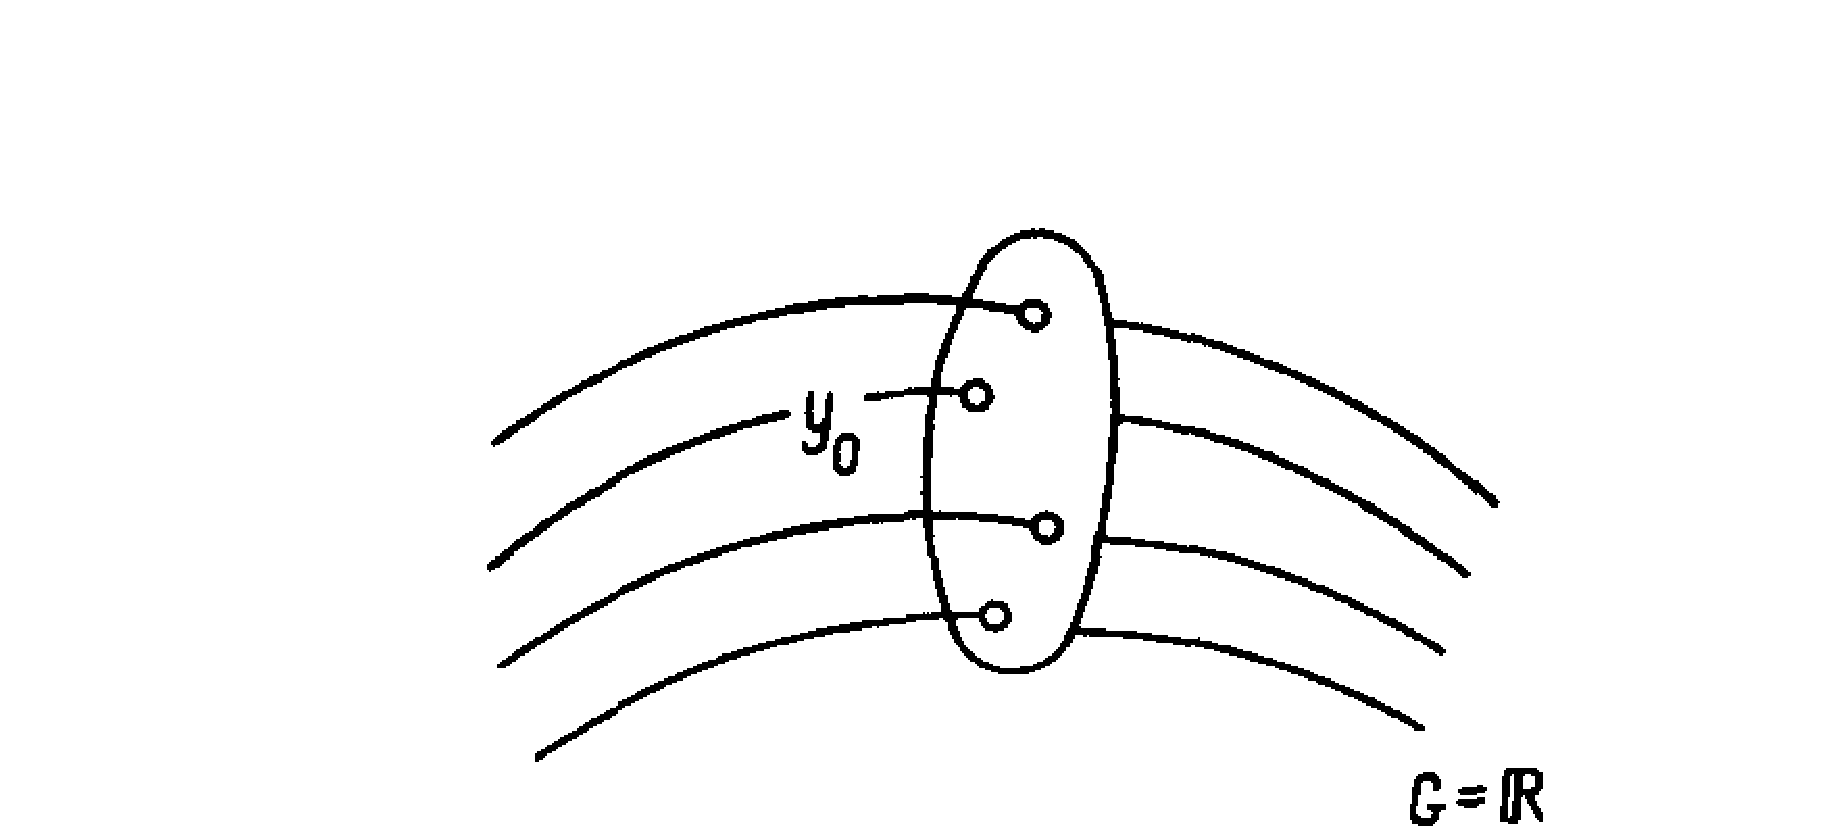
\includegraphics[width=0.62\textwidth]{figures/fig3_8.png}
\end{center}
\figtitle{3.8}{$F=G=\R$ 的情形：把群 $G$ 实现为自身的（右）平移变换群，即主丛的典范构造}

「障碍」概念在代数拓扑中具有根本的重要性；它最初正是为回答下述问题而产生的。

\para{问题 1.} 设 $L$ 是复形 $K$ 的子复形，$f:L\to X$ 是从 $L$ 到任意拓扑空间 $X$ 的映射。如果 $f$ 能延拓，它如何延拓到整个 $K$ 上？又设 $f_\alpha:K\to X$（$\alpha=1,2$）是两个映射，$F:L\times I\to X$ 是这两个映射在子复形 $L$ 上的限制之间的一个同伦。同伦 $F$ 能否延拓到整个 $K$ 上，即延拓为 $f_1$ 与 $f_2$ 之间的同伦？

\para{问题 2.} 设 $p:E\to B$ 是纤维丛（底空间 $B$ 为单纯复形或 CW 复形），$\psi:L\to E$ 是该丛在子复形 $L\subset B$ 上的截面：$p\psi=1_L$。怎样把截面延拓到整个 $B$ 上？两个截面的同伦的类似问题是：给定 $B$ 上的两个截面以及它们在 $L\subset B$ 上的一个同伦，怎样把这个同伦延拓为原来的两个截面之间的同伦，即在 $B$ 的全部上的同伦？

\para{问题 3.} 设 $(E,B,F,G,p)$ 与 $(E',B',F,G,p')$ 是有相同纤维与结构群的纤维丛，$L\subset B$ 是如上所述的子复形，$f:L\to B'$ 是诱导出纤维丛映射 $f:p^{-1}(L)\to E'$ 的映射。怎样把映射 $f$ 延拓为纤维丛映射 $E\to E'$？两个纤维丛映射之间的同伦也有类似的问题。

我们从第一个问题开始。于是，我们要把映射 $f:L\to X$ 从子复形 $L\subset K$ 延拓到整个 CW 复形 $K$。归纳地设 $f$ 已在所有维数 $\le n-1$ 的胞腔上有定义。这样，若 $\sigma^n_\alpha$ 是 $K$ 中不含于 $L$ 的任一胞腔，则假定 $f$ 已在其边界 $\partial\sigma^n_\alpha$ 上有定义：
\[
f|_{\partial\sigma^n_\alpha}:\partial\sigma^n_\alpha\longrightarrow X.
\]

% [原文 p.83]
显然，该映射能延拓到 $\sigma^n_\alpha$ 的内部，当且仅当球面映射 $S^{n-1}_\alpha\overset{\cong}{\longrightarrow}\partial\sigma^n_\alpha\xrightarrow{f|_{\partial\sigma^n_\alpha}}X$ 是零伦的。无论如何，映射 $S^{n-1}_\alpha\to X$ 决定一个元素
\[
\lambda(\sigma^n_\alpha)\in\pi_{n-1}(X).
\]
于是，只要 $n\ge 2$，考虑所有不含于 $L$ 的 $n$-胞腔 $\sigma^n_\alpha$，便得到一个相对上链
\[
\lambda(f)\in C^n(K,L;\pi_{n-1}(X)),
\]
称为 $f$ 的延拓的一个\emph{障碍}。显然，映射 $f$ 能从 $K$ 的 $(n-1)$-骨架延拓到 $n$-骨架，当且仅当 $\lambda(f)\equiv 0$。

% [Tutor Note: 障碍上链 $\lambda(f)$ 属于 $C^n$，但其系数群是 $\pi_{n-1}(X)$，次数与下标相差 1；这个「错位」是障碍论的系统约定，后文式 (6.6) 与定理 6.1 处还会出现同样的错位。]

然而，有可能在 $(n-1)$-骨架 $K^{n-1}$ 上改变映射 $f$，而保持它在 $(n-2)$-骨架 $K^{n-2}$ 上以及在 $L$ 上不变。注意，$f$ 在每个 $(n-1)$-胞腔 $\sigma^{n-1}_\beta$ 上的限制 $f|_{\sigma^{n-1}_\beta}$ 可以换成另一个映射 $g$：它在 $K^{n-2}\cup L$ 上与 $f$ 一致，但在不含于 $L$ 的胞腔 $\sigma^{n-1}_\beta$ 的内部与 $f$ 不同。由于 $f$ 与 $g$ 在每个这样的胞腔的边界 $\partial\sigma^{n-1}_\beta$ 上一致，它们决定一个映射 $S^{n-1}\to X$，代表一个同伦类（「区分元素」）$\mu(\sigma^{n-1}_\beta)\in\pi_{n-1}(X)$。把所有这样的胞腔 $\sigma^{n-1}_\beta$ 都计入，便得到一个相对 $(n-1)$-上链
\[
\mu(f)\in C^{n-1}(K,L;\pi_{n-1}(X)).
\]
通过诱导同态 $f_*:\pi_1(L)\to\pi_1(X)$，同伦群 $\pi_j(X)$ 获得 $\Z[\pi_1(L)]$-模结构，于是上链复形 $C^*(K,L;\pi_{n-1}(X))$ 也获得 $\Z[\pi_1(L)]$-模结构。以下假定 $\pi_1(L)\cong\pi_1(K)=\pi$（经由同态 $f_*:\pi_1(L)\to\pi_1(K)$），且映射 $f$ 已在 $K$ 的 $(n-2)$-骨架上有定义。此时下述断言成立：

\begin{enumerate}[label=(\roman*),leftmargin=2.2em]
\item 障碍上链 $\lambda(f)$ 是把 $C^*(K,L;\pi_{n-1}(X))$ 看作 $\Z[\pi]$-模复形时的上闭链：$\partial^*(\lambda(f))=0$。
\item 把映射 $f$ 在 $K$ 的 $(n-1)$-骨架中不含于 $L$ 的那一部分上改变（例如改成映射 $g$），而保持它在 $(n-2)$-骨架上不变（即 $f=g$ 于 $K^{n-2}\cup L$ 上），将使障碍上闭链 $\lambda(f)$ 改变一个任意的上边缘：
\[
\lambda(f)\longmapsto\lambda(f)+\partial^*(\mu),
\]
其中 $\mu\in C^{n-1}(K,L;\pi_{n-1}(X))$，而 $\partial^*$ 是上边缘同态：$\partial^*:C^{n-1}(K,L;\pi_{n-1}(X))\to C^n(K,L;\pi_{n-1}(X))$。
\end{enumerate}

由此我们断言：

要把给定的映射 $f$ 延拓到 $K$ 的 $n$-骨架，同时保持它在 $(n-2)$-骨架上不变（但允许 $f$ 在 $(n-1)$-骨架中不含于 $L$ 的那一部分上改变），其充要条件是：$\Z[\pi]$-模复形 $C^*(K,L;\pi_{n-1}(X))$ 中的障碍上同调类 $[\lambda(f)]$ 为零：
% [原文 p.84]
\[
0=[\lambda(f)]\in H^{n-1}(K,L;\pi_{n-1}(X)).
\]

允许 $f$ 在维数 $\le n-2$ 的胞腔（不含于 $L$ 者）上改变，会带来更复杂的改变障碍上链 $\lambda(f)$ 的规则。特别地，由 $f$ 在 $(n-2)$-骨架上的改变所引起的 $\lambda(f)$ 的改变，可以完全用「上同调运算」来描述（上同调运算是在 20 世纪 40 年代与 50 年代初由 Pontryagin、Steenrod、Postnikov、Boltyanskii 与 Liao 引入的）；这些上同调运算我们将在下文考虑。

注意，若复形 $K$ 单连通（或同态 $f_*:\pi_1(L)\to\pi_1(X)$ 平凡），则障碍类 $[\lambda(f)]$ 落在以群 $\pi_{n-1}(X)$ 为系数的通常相对上同调群中。

同伦延拓的相应问题可化归为上述映射延拓问题：取 $K_1=K\times[a,b]$，并令 $L_1\subset K_1$ 由顶盖与底盖组成：
\[
K_1=K\times[a,b],\qquad L_1=(K\times\{a\})\cup(K\times\{b\}).
\]
给定的映射 $f_1:L_1\to X$ 由两个给定映射 $f_a:K\to X$、$f_b:K\to X$ 定义。设我们已把同伦 $L\times I\to X$ 延拓到 $K$ 的 $(n-1)$-骨架上（$n\ge 3$），从而有 $F:(K^{n-1}\cup L)\times I\to X$。照上面的论证，可以把同伦 $F$ 延拓到 $K^n$ 的障碍提炼为一个元素
\[
\lambda\in C^{n+1}(K_1,L_1;\pi_n(X)),\qquad n\ge 3.
\]
由此可见，把同伦 $F$ 延拓到 $K$ 的 $n$-骨架的障碍，由 $\lambda$ 的上同调类代表，或等价地由相应元素
\[
[\lambda]\in H^{n+1}(K_1,L_1;\pi_n(X))\cong H^n(K;\pi_n(X))
\]
代表，其中上同调群是就 $\Z[\pi]$-模复形
\[
C^*(K;\pi_n(X)),\qquad C^*(K_1,L_1;\pi_n(X)),\qquad \pi=\pi_1(K)
\]
定义的。

上述延拓问题中的第二个可类似处理：设截面 $\psi$ 在 $L$ 上已定义，并已定义在底空间 $B$ 的 $(n-1)$-骨架 $B^{n-1}$ 上，我们要把它从每个 $n$-胞腔 $\sigma^n_\alpha$ 的边界 $\partial\sigma^n_\alpha$ 延拓到该胞腔的内部。已知的限制映射
\[
\psi|_{\partial\sigma^n_\alpha}:\partial\sigma^n_\alpha\longrightarrow E,\qquad p\psi=1,
\]

% [原文 p.85]
决定 $(n-1)$-球面的一个映射
\[
S^{n-1}\longrightarrow\partial\sigma^n_\alpha\xrightarrow{\ \psi\ }p^{-1}(\sigma^n_\alpha)\cong\sigma^n_\alpha\times F,
\]
后者又决定群 $\pi_{n-1}(F)$ 的一个元素。

注意，$\pi_1(B)$ 在纤维上的作用（由纤维丛上的「同伦联络」决定，见第 2 章 §3）诱导出 $\pi_1(B)$ 在 $\pi_j(F)$ 上的作用，把后者变成 $\Z[\pi_1(B)]$-模。于是，和前面十分类似，出现截面 $\psi$ 延拓的一个障碍上同调类：
\[
[\lambda]\in H^n(B;\pi_{n-1}(F)),
\]
其中上同调群 $H^j(B;\pi_{n-1}(F))$ 是就 $\Z[\pi_1(B)]$-模复形 $C^*(B;\pi_{n-1}(F))$ 定义的。若允许 $\psi$ 在 $B$ 中不含于 $L$ 的 $(n-1)$-胞腔上改变，而保持它在 $B^{n-2}\cup L$ 上不变，则和前面一样，障碍上闭链 $\lambda$ 可以换成同一个上同调类 $[\lambda]$ 中的任何其它上闭链。

两个截面之间的同伦的障碍理论类似：把同伦从 $B^{n-1}$ 延拓到 $B^n$ 的障碍类，是群 $H^n(B;\pi_{n-1}F)$ 的一个元素。

第三个问题的处理与前两个类似，只有一点差别。设我们已有丛映射 $\Phi_{n-1}:p^{-1}(B^{n-1}\cup L)\to E'$，定义在 $E$ 中位于 $B^{n-1}\cup L$（$L\subset B$）上方的部分上，它决定两个底空间的 $(n-1)$-骨架之间的映射 $\phi:B^{n-1}\to B'^{n-1}$。于是可以定义把 $\Phi_{n-1}$ 延拓为 $B^n$ 上方的丛映射 $\Phi_n$ 的障碍。不过，适宜的做法是只对\emph{主丛}（即 $F=G$，$G$ 为两个纤维丛的结构群）考虑这个问题，因为这类障碍的理论可化归为相伴主丛的情形。

在主 $G$-丛的底空间 $B$ 的每个胞腔 $\sigma^n_\alpha$ 上方，和通常一样有
\[
p^{-1}(\sigma^n_\alpha)\cong\sigma^n_\alpha\times G.
\]
$\Phi_{n-1}$ 在 $\partial(\sigma^n_\alpha)\times\{1\}$ 上的限制（它覆盖 $\phi|_{\partial(\sigma^n_\alpha)}$，其中 $1$ 是 $G$ 的单位元）决定一个从 $(n-1)$-球面到 $E'$ 的映射：
\[
S^{n-1}\cong\partial(\sigma^n_\alpha)\times\{1\}\xrightarrow{\ \Phi_{n-1}\ }E',
\]
\[
p'\circ\Phi_{n-1}|_{\partial(\sigma^n_\alpha)\times\{1\}}=\phi|_{\partial(\sigma^n_\alpha)}.
\]
这样决定的映射 $S^{n-1}\to E'$ 定义了 $\pi_{n-1}(E')$ 的一个元素；把所有 $\phi$ 尚未在其上有定义的胞腔 $\sigma^n_\alpha$ 都计入，便得到取值于 $\pi_{n-1}(E')$ 的障碍上链 $\lambda$。相应的上链复形可以通过诱导同态
\[
\phi_*:\pi_1(B)\longrightarrow\pi_1(B')
\]
拉回 $\pi_1(B')$ 的作用，从而获得 $\Z[\pi_1(B)]$-模结构。

% [原文 p.86]
若 $B$ 单连通，则和前面一样，障碍类属于以群 $\pi_{n-1}(E')$ 为系数的通常上同调群。由此可以推出关于上述三个问题的下述结论：

\emph{若问题 1 中空间 $X$（或问题 2 中的纤维 $F$，或问题 3 中的全空间 $E'$）的同伦群在维数 $\le n$ 时平凡，则对于维数 $\le n$ 的 CW 复形 $K$（以及问题 2、3 中的底空间 $B$），任何定义在 $K$（或 $B$）的维数 $\le n$ 的骨架上的映射（问题 2 中的截面、问题 3 中的丛映射）都能延拓到下一维的骨架上；对定义在维数 $\le n-1$ 的骨架上的同伦（其含义按三个问题各自的意义理解）亦然。}

作为特例立即得到：对任何纤维丛 $(E,B,F,G,p)$，到相应万有丛的丛映射
\[
\Phi:(E,B,F,G,p)\longrightarrow(E',B',F,G,p')
\]
在同伦意义下只有一个，因为全空间 $E'$ 可缩。按标准记法把万有丛的底空间记作 $B'=B_G$，便可推出：每个纤维丛 $(E,B,F,G,p)$ 都决定一个映射 $f:B\to B_G$，它在同伦意义下唯一（反过来，这个映射从万有丛诱导出给定的纤维丛）。这样的同伦当然是映射 $f:B\times I\to B_G$，从而在柱体 $B\times I$ 上诱导出一个纤维丛。由于柱体 $B\times I$（$I=[a,b]$）可以收缩到它的底 $B\times\{a\}$，并使顶盖 $B\times\{b\}$「恒等地」变到 $B\times\{a\}$ 上（即对一切 $x\in B$ 有 $(x,b)\mapsto(x,a)$），故对任何系数群都有 $H^j(B\times I,B\times\{a\})=0$。由此可见，$B\times I$ 上的任何纤维丛都可以映射到基 $B\times\{a\}$ 上的限制丛，并使底空间的诱导映射把 $B\times I$ 的顶盖 $B\times\{b\}$「恒等地」送到 $B\times\{a\}$。为了得出我们想得到的结论，先需要一个预备定义。

\begin{definition*}{6.2}
设两个纤维丛有相同的底空间 $B$、相同的纤维 $F$ 与相同的结构群 $G$。若它们之间存在一个在公共底空间上诱导恒等映射的丛映射
\[
\Phi:(E,B,F,G,p)\longrightarrow(E',B,F,G,p'),
\]
则称这两个纤维丛是\emph{等价的}。
\end{definition*}

上述讨论归结为下述重要结果。

\begin{theorem*}{6.1}
以 $B$ 为底空间、$F$ 为纤维、$G$ 为结构群的纤维丛的等价类集合，与底空间 $B$ 到相应万有丛底空间 $B_G$ 的映射的同伦类集合之间，存在自然的一一对应。
\end{theorem*}

% [Tutor Note: 定理 6.1 说的是两个集合之间的一一对应，不是群同构；$B_G$ 即通常所说的分类空间，第 4 章讨论示性类时会给出它的具体模型（Grassmann 流形）。]

\begin{example}{1}
由万有主 $G$-丛（$F=G$）的正合同伦列（见第 2 章 (4.7)），并计入全空间的可缩性，可得如下同构：

% [原文 p.87]
\begin{equation}
\pi_n(B_G)\cong\pi_{n-1}(G)\ (=\pi_{n-1}(F)),\qquad n\ge 1. \tag{6.4}
\end{equation}
这个同构与前述定理一起表明：以 $S^n$ 为底的 $G$-丛的等价类，由群 $\pi_{n-1}(G)$ 分类。回忆一下：对拓扑群 $G$，含单位元的连通分支 $G_0$ 是正规子群，故 $\pi_0(G)=G/G_0$ 具有自然的群结构；于是可以推知，$\pi_1(B_G)$（$\cong\pi_0(G)$）在群 $\pi_n(B_G)$（$\cong\pi_{n-1}(G)$）上的作用，等同于 $\pi_0(G)$ 在 $\pi_{n-1}(G)$ 上的作用：
\begin{equation}
q(a)=qaq^{-1},\qquad q\in\pi_0(G),\ a\in\pi_{n-1}(G). \tag{6.5}
\end{equation}
因此，映射 $S^n\to B_G$ 的自由同伦类（即不区分基点的同伦类）与 $\pi_{n-1}(G)$ 在由 (6.5) 给出的 $\pi_0(G)$ 作用下的轨道之间，存在自然的一一对应；于是可以用这些轨道来确定 $S^n$ 上互不等价的 $G$-丛。

从几何上说，把 $S^n$ 上 $G$-丛的分类问题化归为对群 $\pi_{n-1}(G)$ 的考察，是非常自然的：把球面 $S^n$ 看作两个半球 $D^n_+\cup D^n_-$ 的并，其边界（赤道）等同。由于两个半球都可缩，$S^n$ 上的任何 $G$-丛在每个半球上都平凡。于是有结构同胚
\[
\phi_1:p^{-1}(D^n_+)\longrightarrow D^n_+\times G,
\]
\[
\phi_2:p^{-1}(D^n_-)\longrightarrow D^n_-\times G
\]
（这里假定 $G$-丛是主丛），而赤道上的衔接函数
\[
\lambda_{12}=\phi_1\phi_2^{-1}:S^{n-1}\times G\longrightarrow S^{n-1}\times G
\]
具有形状
\[
\lambda_{12}(x,g)=(x,\hat\lambda_{12}(x)(g)),
\]
其中 $\hat\lambda_{12}:S^{n-1}\to G$ 代表 $\pi_{n-1}(G)$ 中适当的同伦类。
\end{example}

% [Tutor Note: 原书 p.87 与 p.88 各有一个『例 1』，编号重复，系原书排版之误；译文照原书保留，引用时务必分清：p.87 的例 1 给出式 (6.4)，p.88 的例 1 才是求解 Hopf 分类问题的那个。]

上述分类定理的最终形式看来是由 Steenrod 给出的，不过此前 Pontryagin、Ehresmann、Chern 等人已在涉及某些重要的特殊万有丛的方向上作过研究。至于障碍，这一概念的一个版本最早出现于 20 世纪 30 年代初，与 Van Kampen 关于 $n$ 维复形 $K^n$（$n\ge 2$）的构造有关：这些复形是 Euler 三宅三井问题中出现的 1 维复形的高维类似物，其意是指它们不能无自交地嵌入 $\R^{2n}$。这一思想后来由 Whitney 加以发展，特别是用于纤维丛的截面；Pontryagin 与 Whitehead 又把它积极用于同伦论的具体问题。显然，障碍概念的这种最终表述，在映射的情形归功于 Eilenberg，在纤维丛的情形归功于 Steenrod。

% [原文 p.88]
顺带指出，纤维可缩的纤维丛有截面，而且这些截面彼此都同伦。这种情形将在光滑流形论中频繁出现，第 4 章专门讨论它。

在具体的拓扑问题中，最常用的是所谓\emph{第一障碍}。它就是试图把映射（上述问题 1）或丛的截面（问题 2）从相应空间的 $(n-1)$-骨架延拓到 $n$-骨架时出现的障碍，其中 $n$ 是使目标空间 $X$ 的同伦群（问题 1）首次非平凡的维数：
\[
\pi_n(X)\ne 0,\qquad \pi_j(X)=0\quad\text{对 } j<n,
\]
或者使纤维 $F$ 的同伦群（问题 2）首次非平凡的维数：
\[
\pi_n(F)\ne 0,\qquad \pi_j(F)=0\quad\text{对 } j<n.
\]

\begin{example}{1}
考虑 Hopf 问题：把 $n$ 维 CW 复形 $K^n$ 到 $n$-球面 $S^n$ 的映射按同伦分类。这里映射的延拓没有障碍。同伦的延拓恰有一个障碍，它位于群 $H^n(K^n;\Z)$ 中，因为 $\pi_n(S^n)\cong\Z$。由此可知，映射 $K^n\to S^n$ 的同伦类与群 $H^n(K^n;\Z)$ 的元素之间自然一一对应。等价地，这些同伦类与 $K^n$ 与 $S^n$ 的第 $n$ 个整同调群之间的同态一一对应，因为
\[
H^n(K^n;\Z)=\Hom(H_n(K^n;\Z),\Z),\qquad \Z\cong H_n(S^n;\Z).
\]
\end{example}

\begin{example}{2}
上一例可以（略微）推广：把 $S^n$ 换成任何 $(n-1)$-连通空间 $X$（即满足 $\pi_j(X)=0$（$j<n$）的空间）。于是要分类 $n$ 维 CW 复形 $K^n$ 到 $X$ 的映射的同伦类。如前，由于 $(n-1)$-连通性，只有第一障碍出现，并得到类似结果：每个映射 $K^n\to X$ 在同伦意义下由 $H^n(K^n;\pi_n(X))$ 中唯一的上同调类决定；等价地，由 $K^n$ 与 $X$ 的第 $n$ 个整同调群之间唯一的同态决定，因为
\[
H^n(K^n;\pi_n(X))=\Hom(H_n(K^n;\Z),H_n(X;\Z)),\qquad H_n(X;\Z)\cong\pi_n(X).
\]
\end{example}

\begin{example}{3}
设 $X$ 是 $K(\pi,n)$ 型的 Eilenberg--MacLane 空间，即
\[
\pi_n(X)\cong\pi,\qquad \pi_j(X)=0\quad\text{对 } j\ne n.
\]

% [原文 p.89]
前两个例子的论证导致同样的结论，只是这里对任何 CW 复形 $K$ 都成立：映射 $K\to X$ 的同伦类集合与 $H^n(K;\pi)$ 自然一一对应，因此，只要 $n>1$，它就获得 Abel 群的结构。由于 $H_n(K(\pi,n);\Z)\cong\pi_n(K(\pi,n))\cong\pi$，且
\[
H^n(K(\pi,n);\pi)\cong\Hom(H_n(K(\pi,n);\Z),\pi)\cong\Hom(\pi,\pi),
\]
$H^n(K(\pi,n);\pi)$ 中有一个对应于恒等同构 $1:\pi\to\pi$ 的特定元素 $u$，称为 $H^n(K(\pi,n);\pi)$ 的\emph{基本类}。用基本类 $u$ 表述，映射 $f:K\to K(\pi,n)$ 的同伦类 $[f]$ 与 $H^n(K;\pi)$ 的元素之间的上述对应由
\begin{equation}
[f]\longmapsto f^*(u)\in H^n(K;\pi) \tag{6.6}
\end{equation}
给出。注意，当 $n=1$ 时，上述结论对非 Abel 群 $\pi$ 也成立，因为如前所述，对这种 $\pi$，$H^1(K;\pi)$ 仍有定义（作为集合）。由 (6.6) 可以断言：

$K(\pi,n)$ 型的 Eilenberg--MacLane 空间对于以 $\pi$ 为系数的 $n$ 维上同调类的分类是万有的（正如主万有 $G$-丛对 $G$-丛等价类的分类是万有的）。

如前所述，对于 $K(\pi,1)$ 型的 Eilenberg--MacLane 复形我们已知一系列例子，还有 $K(\Z,2)=\CP^\infty$（$=\lim\limits_{n\to\infty}\CP^n$）；至于其余的，我们只知道它们存在。凭借 (6.6)，这些复形在拓扑学中起着重要的技术作用。
\end{example}

\begin{definition*}{6.3}
\emph{上同调运算}是指 $k$ 个变量 $z_j\in H^{n_j}(X;G_j)$ 的一个「自然」函数 $\theta_X(z_1,\dots,z_k)$，取值于 $H^*(X;G)$。这里「自然」意味着该运算应当是函子性的，即与映射 $f:Y\to X$ 诱导的同态交换：
\begin{equation}
\text{若 } f^*(z_j)=z'_j,\quad\text{则}\quad \theta_Y(z'_1,\dots,z'_k)=f^*\theta_X(z_1,\dots,z_k). \tag{6.7}
\end{equation}
\end{definition*}

最简单的例子是任意 $k$ 个元素的乘积 $\theta=z_1\cdots z_k$，其中所有 $G_j=G$。然而重要的是：确实存在只含一个变量的上同调运算 $\theta(z)$，它们不能仅用 $H^*(X;G)$ 的环结构来定义，在 $G=\Z/p$ 的情形尤其如此。最简单的这类「非平凡」例子是 Bockstein 同态（见 §4）
\[
\beta:H^q(X;\Z/p)\longrightarrow H^{q+1}(X;\Z/p).
\]
鉴于上面指出的 Eilenberg--MacLane 空间在上同调类分类方面的万有性质，上述形状的全部上同调运算与元素
\[
\theta\in H^*(K(G_1,n_1)\times\cdots\times K(G_k,n_k);G)
\]
自然一一对应。

% [原文 p.90]
这个对应用基本类来定义很方便（见 (6.6)）：
\[
u_j\longmapsto 1_{G_j},\qquad H^{n_j}(K(G_j,n_j);G_j)\cong\Hom(G_j,G_j),
\]
于是
\begin{equation}
\theta=\theta(u_1,\dots,u_k). \tag{6.8}
\end{equation}
对给定的空间 $X$ 与元素 $z_j\in H^{n_j}(X;G_j)$（$j=1,\dots,k$），存在映射 $f_j:X\to K(G_j,n_j)$ 使得 $z_j=f^*(u_j)$，由此得到映射
\[
f=f_1\times\cdots\times f_k:X\longrightarrow K(G_1,n_1)\times\cdots\times K(G_k,n_k),
\]
而运算 $\theta$ 在 $(z_1,\dots,z_k)$ 上的值 $\theta_X(z_1,\dots,z_k)\in H^*(X;G)$ 由
\[
\theta_X(z_1,\dots,z_k)=f^*\theta(u_1,\dots,u_k)
\]
给出。（这是 Serre 在 20 世纪 50 年代初注意到的。）

除运算 $\beta$ 之外，人们更早还发现了其它一些特殊的非平凡上同调运算：

\begin{enumerate}[label=\arabic*),leftmargin=2em]
\item Pontryagin 平方与幂：
\[
\mathcal{P}_p:H^{2q}(X;\Z/p)\longrightarrow H^{2pq}(X;\Z/p^2),
\]
其中 $\mathcal{P}_p(z)\equiv z^p\bmod p$，$p$ 为素数。
\item Steenrod 平方与幂：
\begin{enumerate}[label=\alph*),leftmargin=1.8em]
\item Steenrod 平方：
\[
Sq^i:H^q(X;\Z/2)\longrightarrow H^{q+i}(X;\Z/2),
\]
其中特别地 $Sq^0=1$，而 $Sq^1$ 是 $p=2$ 时的 Bockstein 同态；
\item Steenrod 幂：
\[
St^i_p:H^q(X;\Z/p)\longrightarrow H^{q+i}(X;\Z/p),
\]
其中特别地 $St^0_p=1$，而 $St^1_p$ 与 Bockstein 算子 $\beta$ 一致。
\end{enumerate}
\end{enumerate}

Steenrod 平方是同态，并且具有下述进一步的基本性质：
\begin{enumerate}[label=(\roman*),leftmargin=2.2em]
\item $Sq^0=1$，$Sq^1=\beta$，$Sq^n(z)=z^2$，$z\in H^n(X;\Z/2)$。
\item Steenrod 平方是\emph{稳定的}，即它们与悬挂同构
\[
E:H^q(X;\Z/2)\longrightarrow H^{q+1}(\Sigma X;\Z/2)
\]
交换。
\end{enumerate}
% CHUNK ch03f DONE
